\documentclass[a4paper]{article}

\usepackage[utf8]{inputenc}
\usepackage[ngerman]{babel}
\usepackage[T1]{fontenc}

\usepackage{amsmath}
\usepackage{amssymb}
\usepackage{siunitx}
\usepackage{graphicx}

% IHK Richtlinien
\usepackage{timesnew}
\usepackage[top=3.5cm, bottom=2.5cm, left=3.5cm, right=2.5cm]{geometry}


\title{Projektarbeit 1. Lehrjahr\\Leistungs-, Spannungs- und Stromanpassung}

\author{Henning Meyer\\Erik Bauer}


\begin{document}
\pagenumbering{gobble}

%TODO Titelseite gestalten

\maketitle
\begin{center}
    
\includegraphics[width=6cm]{img/logo}
\end{center}
\newpage
\tableofcontents
\newpage

% Anfang der Arbeit
\pagenumbering{arabic}

% IHK Richtlinien
\fontencoding{T1}
\fontfamily{times}
\fontsize{11}{14}
\selectfont

\section{Analyse und Vorüberlegungen}

\subsection{IST-Analyse}

\subsubsection{Situation des Auftraggebers}

    Der Auftraggeber für dieses Projekt ist die technische Berufsschule Rostock.
    Die Schule besitzt mehrere Laborräume, in denen Computer mit gängiger Peripherie wie Maus und Tastatur vorhanden sind.
    Diese werden in gegebenen Unterrichtsstunden den Schülern zum Arbeiten zur Verfügung gestellt.
    Auf den Computern befinden sich u.a. Entwicklungsumgebungen für verschiedene Programmiersprachen, darunter die für dieses Projekt relevante Software \glqq Microsoft Visual Studio\grqq{} in verschiedenen Versionen.
    Die Rechner verfügen ebenfalls über einen Internetzugang für Recherchezwecke, Anbindung an das lokale Schulnetzwerk mit Speicherplatz für jeden Schüler, sowie Schutzsoftware, um die Funktionalität der lokalen PCs zu gewährleisten.

\subsubsection{Situation des Auftragsnehmers}

    Der Auftragsnehmer ist in Form eines Projektteams bestehend aus zwei Schülern der Klasse FIN81 gegeben.
    Beide absolvieren das erste Lehrjahr der Ausbildung zum Fachinformatiker für Anwendungsentwicklung.
    Es bestehen auf beiden Seiten Vorkenntnisse in der Programmierung in unterschiedlichen Programmiersprachen.

    Herr Meyer ist vor allem im Bereich der Webprogrammierung tätig, wobei er mit Hilfe von \glqq ASP.NET\grqq{} Webseiten bearbeitet.
    Daraus resultierend ist er vertraut mit den Programmiersprachen \glqq C\#\grqq{} und \glqq Javascript\grqq{}, sowie den Auszeichnungssprachen \glqq HTML5\grqq{} und \glqq CSS3\grqq{}.

    Herr Bauer hat ebenfalls bereits Erfahrung in der Programmierung mit \glqq Javascript\grqq{} und \glqq C\#\grqq{}, sowie den Sprachen \glqq Python\grqq{} und \glqq C\grqq{}.

    Zum Arbeiten besitzen die Teammitglieder eigene Computer, es stehen ihnen aber ggf. auch Rechner in ihren Arbeitsplätzen und in der Berufsschule zur Verfügung.

\subsection{SOLL-Analyse}

    Als Anforderung an das Projektteam wurden Kriterien für ein Programm, sowie eine dazugehörige schriftliche Ausarbeitung gegeben.
    Die gewünschte Anwendung ist hierbei durch Muss-/ und Wunsch-Funktionalitäten beschrieben, konkrete Einschränkungen an die Umsetzung sind dabei aber nicht gemacht worden.
    Die Hauptaufgabe des Programms liegt in der Visualisierung von physikalischen Messdaten und deren Zusammenhänge in Form von dynamisch erstellten Graphen.
    Außerdem muss es zu Präsentationszwecken auf den Schulrechnern lauffähig sein.

\subsection{Problemstellung}

    Es ist eine Beschreibung einer elektrotechnischen Schaltung gegeben. Die mathematischen Zusammenhänge zwischen den physikalischen Größen, sind vom Programm automatisch als Graph darzustellen. Speziell soll der Graph in einem begrenzten Maße ohne Nutzung fremden Quellcodes gezeichnet werden. Des Weiteren sind die Graphen nur als Näherungskurve darzustellen.

    \subsubsection{Begriffsdefinitionen}

    \begin{itemize}
        \item[Spannung]
        Die elektrische Spannung mit dem Formelzeichen $U$ und der Einheit Volt ($\si{\volt}$), beschreibt die Eigenschaft, Ladung zu bewegen.
        Sie ist Ursache für das Fließen eines elektrischen Stroms innerhalb eines elektrisch leitfähigen Elementes.
        \item[Stromstärke]
        Die elektrische Stromstärke besitzt das Formelzeichen $I$ und die Einheit Ampere ($\si{\ampere}$).
        Sie bemisst den elektrischen Strom im Bezug auf eine gegebene Fläche, zum Beispiel der Querschnittfläche eines Leiters oder Kondensators.
        \item[Widerstand]
        Der elektrische Widerstand, welcher durch das Formelzeichen $R$ und die Einheit Ohm ($\si{\ohm}$) gekennzeichnet wird, gibt an, welche elektrische Spannung notwendig ist, um eine bestimmte elektrische Stromstärke durch einen elektrischen Leiter zu transportieren.
        \item[Leistung]
        Das Formelzeichen $P$ und die Einheit Watt ($\si{\watt}$) beschreiben die Leistung im generellen Sinne.
        Die elektrische Leistung beschreibt die Arbeit, welche ein elektrischer Strom in einer bestimmten Zeit verrichtet bzw. die Energie, welche in dieser Zeitspanne umgesetzt wird.
        \item[Spannungsanpassung]
        Unter Spannungsanpassung versteht man die Optimierung der Beziehung zwischen elektrischer Spannungsquelle und elektrischem Verbraucher einer elektrischen Schaltung zugunsten der elektrischen Spannung.
        Es soll die maximale elektrische Spannung am Verbraucher erreicht werden.
        Dies geschieht, wenn der Widerstand außerhalb der Spannungsquelle größer ist, als innerhalb der Spannungsquelle.
        \item[Stromanapassung]
        Unter Stromanpassung versteht man die Optimierung einer elektrischen Schaltung zugunsten des elektrischen Stroms, wobei die Beziehung zwischen elektrischer Spannungsquelle und elektrischen Verbraucher angepasst wird.
        Ziel ist, die maximale Stromstärke zu erreichen.
        Dazu muss der Widerstand innerhalb der Schaltung den Widerstand außerhalb der Schaltung überwiegen.
        \item[Leistungsanpassung]
        Als Leistungsanpassung wird die Optimierung einer elektrischen Schaltung zugunsten der elektrischen Leistung bezeichnet.
        Der Widerstand der Spannungsquelle muss dabei dem Widerstand am Verbraucher gleichen, um die maximale Leistung zu erreichen.
    \end{itemize}

    \subsubsection{Betrachtung mathematischer Zusammenhänge}

    Da die mathematischen Zusammenhänge klar definiert sind, lassen sich über die im Programm zu erwartenden Ergebnisse einige Vorüberlegungen treffen.
    Sofern zum Berechnen der Werte und zum Zeichnen des Graphen geeignete Algorithmen verwendet werden, sollten die produzierten Ausgaben den definierten Beziehungen entsprechen.

    Gegeben sind eine Spannungsquelle $U_0$ von $10 \si{\volt}$, sowie ein veränderlicher Lastwiderstand $R_L$ im Verbraucher $L$.
    Zu berechnen sind nun die Stromstärke $I_L$, die Stromspannung $U_L$, sowie die elektrische Leistung $P_L$ in Abhängigkeit von $R_L$.

    Die zu erwartenden Veränderungen der unterschiedlichen physikalischen Größen in Abhängigkeit von $R_L$ lassen sich mit Hilfe ihrer Berechnungsformeln herleiten:

    Berechnung von $I_L$:

    \[ I_L = \frac{U_0}{R_L} \]
    \[ I_L = \frac{10\si{\volt}}{R_L} \]

    Berechnung von $U_L$:

    \[ U_L = R_L \cdot I_L \]
    \[ U_L = R_L \cdot \frac{10\si{\volt}}{R_L} \]
    \[ U_L = 10\si{\volt} \]

    Berechnung von $P_L$:

    \[ P_L = U_L \cdot I_L \]
    \[ P_L = 10\si{\volt} \cdot \frac{10\si{\volt}}{R_L} \]
    \[ P_L = \frac{100\si{\volt}}{R_L} \]

    \subsubsection{Wertetabelle und grafische Darstellung im Programm}
    
    Die mathematischen Beziehungen, welche im vorherigen Abschnitt beschrieben wurden, sind im Programm mittels einer Wertetabelle festgehalten und anschließend in einem Graphen visualisiert.
    \begin{figure}[!h]
        \begin{center}
            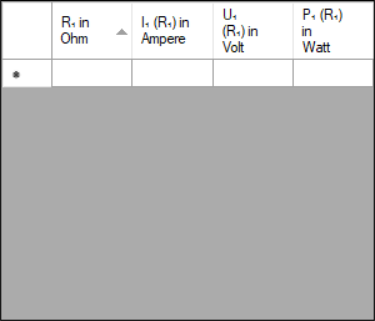
\includegraphics[width=6cm]{img/tabelle}
            \caption{leere Wertetabelle}
            \label{fig:tabelle}
        \end{center}
    \end{figure}

    In Abbildung \ref{fig:tabelle} ist der Initial-zustand der Wertetabelle zu sehen, entsprechend in Abbildung \ref{fig:graph} der Graph in seinem Anfangszustand.
    \begin{figure}[!h]
        \begin{center}
            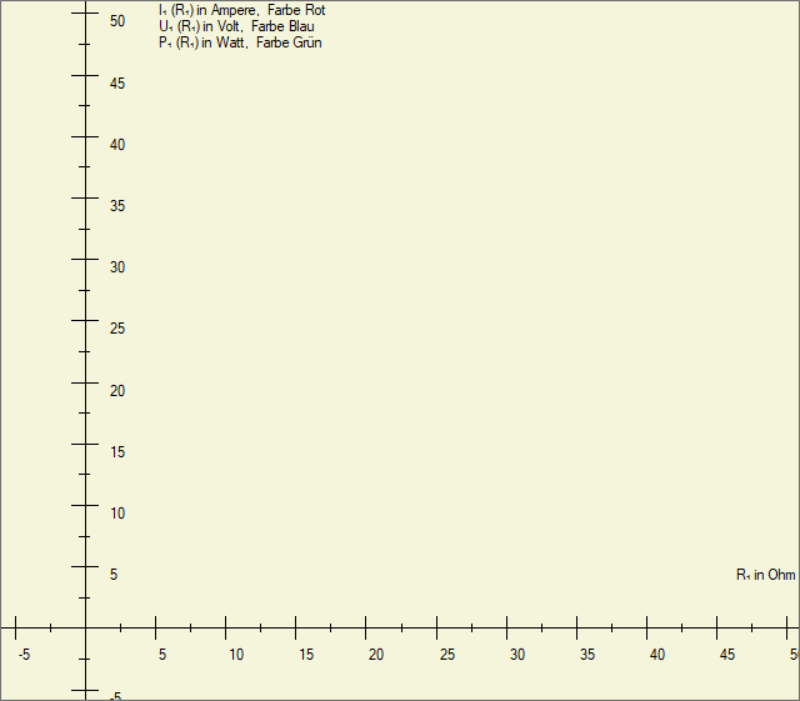
\includegraphics[width=6cm]{img/graph}
            \caption{leerer Graph}
            \label{fig:graph}
        \end{center}
    \end{figure}

    Füllt man nun in die Tabelle einige Widerstandswerte ein, so befüllen sich die abhängigen Werte für Stromstärke, Spannung und Leistung automatisch.
    Zu sehen ist ein befülltes Beispiel in Abbildung \ref{fig:tabellebefuellt}.
    Die Tabelle achtet hierbei darauf, dass keine leeren Felder oder doppelte Widerstandswerte auftreten.
    Sofern keine Werte berechnet bzw. dargestellt werden können, wie zum Beispiel bei einem Widerstand von $0\,\si{\ohm}$, zeigt das Programm ein entsprechendes Symbol für etwa \glqq Unendlich\grqq{}: $\pm\infty$ oder \glqq Nicht definiert\grqq{}: $NaN$.
    \begin{figure}[!h]
        \begin{center}
            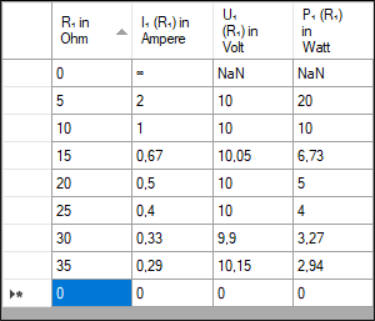
\includegraphics[width=6cm]{img/tabellebefuellt}
            \caption{befüllte Wertetabelle}
            \label{fig:tabellebefuellt}
        \end{center}
    \end{figure}

    Lässt man sich nun den Graphen und die entsprechenden Datenpunkte aus der Wertetabelle darstellen, erhält man ein Bild wie in Abbildung \ref{fig:graphbefuellt} zu sehen ist.
    \begin{figure}[!h]
        \begin{center}
            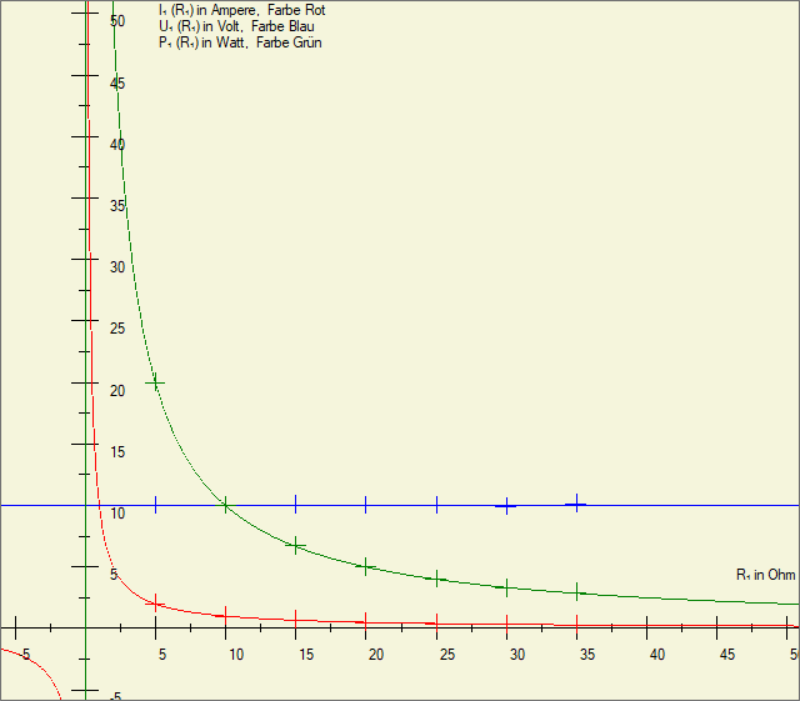
\includegraphics[width=6cm]{img/graphbefuellt}
            \caption{gezeichnete Datenpunkte}
            \label{fig:graphbefuellt}
        \end{center}
    \end{figure}

    \subsubsection{Leistungsanpassung am praktischen Beispiel}
    %TODO Praktisches Beispiel Leistungsanpassung
    
    Leistungsanpassung wird in der Praxis unter anderem bei der Signalübertragung und auch bei der Energiegewinnung in Solarzellen verwendet.

\newpage
\section{Lösungsfindung und Umsetzung}

\subsection{Betrachtung von Lösungsvarianten}

    Nach Analyse der gegebenen Anforderungen entschied das Projektteam, dass eine Entwicklungsumgebung, welche das Erstellen graphischer Oberflächen unterstützt, angemessen zur Lösung ist.
    Außerdem sollte die verwendete Programmiersprache eine einfache Schnittstelle oder Möglichkeit bieten, vom Programmierer definierte Grafiken auf dem Bildschirm anzuzeigen.
    Hierbei sollten speziell einzelne Punkte oder gerade Linien darstellbar sein, damit die Zeichnung von Kurven gut implementierbar ist.
    Als mögliche Programmiersprachen kamen \textit{\glqq Python\grqq{}}, unter Nutzung von \textit{\glqq TKinter\grqq{}}, \textit{\glqq Java\grqq{}} und \textit{\glqq C\#\grqq{}}, sowie \textit{\glqq Javascript\grqq{}} in Frage.
    Zusätzlich zur Seite der Problemstellung, wurde dann die Seite der Vorkenntnisse in Betracht gezogen.
    Mit den gefundenen Kriterien und den Überschneidungen vorhandener Entwicklungserfahrungen, sind sowohl \textit{\glqq Javascript\grqq{}} als auch \textit{\glqq C\#\grqq{}} in die engere Auswahl gekommen.
    Nach dem abwägen möglicher Entwicklungsvorteile und Kompatibilitätskriterien, hat sich das Team letztlich für die Nutzung der Sprache \textit{\glqq C\#\grqq{}}, unterstützt durch die Entwicklungsumgebung \textit{\glqq Microsoft Visual Studio\grqq{}}, entschieden.

\subsection{Umsetzung der gewählten Variante}

    Das Programm ist im Kern modular gestaltet, d.h. jeder funktional eigene Bereich ist durch eine eigene Klasse abgetrennt.
    Die Arbeitsaufteilung wurde dementsprechend auch nach Modulen aufgeteilt.
    Die Erstellung der Wertetabelle wurde von Herr Meyer umgesetzt.
    Die Visualisierung des Graphen hat Herr Bauer übernommen.

    Die Oberfläche des Programms wurde während der funktionalen Entwicklungsphase nur sporadisch gestaltet.
    Überlegungen zum generellen Layout haben zwar schon früh stattgefunden, aber da die einzelnen Bausteine möglichst unabhängig vom Aussehen des Programms funktionieren sollten, wurde der Fokus erst später auf das Design gesetzt.
    Nach einigen Besprechungen, wurde das fertige Layout der graphischen Oberfläche des Programms festgelegt, um eine Orientierung für die Formfaktoren der Bausteine zu bekommen.

    Um den Graphen und die Funktionskurven zu zeichnen wurden verschiedene Methoden implementiert und getestet.
    Anfangs bestand die Idee, die Graphen als Näherungskurven mittels der gegebenen Wertetabelle zu zeichnen, jedoch stellte sich eine geeignete Annäherungsprozedur als zu komplex für die gegebene Aufgabe heraus.
    Besonders, wenn erst wenige Werte eingetragen sind, ist eine Kurve nicht praktikabel anzunähern.
    Daher wird in der finalen Version des Programms eine Repräsentation der mathematischen Zusammenhängen der Werte, in Form von Polynomen, codiert und dargestellt.

    Für die Wertetabelle fanden wir eine geeignete Struktur und konfigurierten diese, bis sie unseren Vorstellungen entsprach.
    Dem Nutzer ist es einfach möglich, neue Widerstands-Werte einzutragen bzw. vorhandene zu löschen.
    Die Werte in Abhängigkeit vom Widerstand werden dann automatisch berechnet.

\newpage
\section{Testen der Anwendung}

\subsection{Betrachtete Testfälle}

    %TODO Testfälle
    \begin{enumerate}
        \item Berechnung der Werte für Ampere, Volt und Watt\\
        \label{test:calc}
        Wenn ein Wert für den Widerstand eingegeben wird, sollen die restlichen in Abhängigkeit vom eingegebenen Wert, Anhand ihrer mathematischen Zusammenhänge, berechnet werden.
        
        \item Darstellung der Datenpunkte aus der Tabelle\\
        \label{test:point}
        Mit eingetragenen Werten in der Tabelle, sollen nach einem Klick auf den Knopf \glqq Zeichne Datenpunkte\grqq{}, die entsprechenden Koordinaten im Graphen visuell hervorgehoben werden.
        
        \item Darstellung der Kurvenverläufe der mathematischen Zusammenhänge\\
        \label{test:curve}
        Durch einen Klick auf den Knopf \glqq Zeichne Graphen\grqq{}, sollen die Kurvenverläufe der drei Funktionen $I_L(R_L)$, $U_L(R_L)$ und $P_L(R_L)$ graphisch dargestellt werden.
        
        \item Löschen der gezeichneten Elemente\\
        \label{test:delete}
        Bei einem Klick auf den Knopf \glqq Lösche Graphen\grqq{}, sollen sämtliche Elemente des Graphen, welche nicht zu den Achsen gehören, gelöscht werden.
        
        %\item Verändern des sichtbaren Koordinatenbereichs\\
        %Nach einem Ändern der Werte für die X-/ Y-Achsenbegrenzung, soll der Graph sich dem neuen Format anpassen und ggf. die gezeichneten Elemente auf die neue Größe skalieren.
    \end{enumerate}

\subsection{Testprotokolle}

    %TODO Testprotokolle
    \begin{center}
        \begin{tabular}[c]{|c|p{100pt}|p{100pt}|p{150pt}|}
            \hline
            Testfall & Durchführung & Erwartung & Ergebnis\\
            \hline
            Nr. \ref{test:calc}
            &
            Mit Ausgang Initial-zustand;\newline
            eintragen von den Widerstandswerten:\newline
            $5$, $10$, $15$, $20$, $3.3$\newline
            in die Tabelle
            &
            Für $I_L(R_L)$:\newline
            $2$, $1$, $0.\overline{3}$, $0.5$, $0.\overline{03}$\newline
            Für $U_L(R_L)$:\newline
            $10$, $10$, $10$, $10$, $10$\newline
            Für $P_L(R_L)$:\newline
            $20$, $10$, $6.\overline{6}$, $5$, $30.\overline{30}$\newline
            &
            Die Werte erscheinen in der Tabelle auf zwei Nachkommastellen gerundet.\newline
            Dadurch treten bei der Spannung vereinzelt Werte auf, welche den Vorüberlegungen geringfügig abweichen.
            \\
            \hline
            Nr. \ref{test:point}
            &
            Mit Ausgang Endzustand von Test Nr. \ref{test:calc};\newline
            betätigen des Knopfes \glqq Zeichne Datenpunkte\grqq{}
            &
            An den Koordinaten mit X-Werten aus der Spalte $R_L$ und Y-Werten aus den übrigen, erscheinen in jeweiliger Farbe Markierungen
            &
            Die Markierungen erscheinen in Form von Kreuzen an den jeweiligen Koordinaten in:\newline
            Rot, für $I_L(R_L)$\newline
            Blau, für $U_L(R_L)$\newline
            Grün, für $P_L(R_L)$\newline
            \\
            \hline
        \end{tabular}
        \begin{tabular}[c]{|c|p{100pt}|p{100pt}|p{150pt}|}
            \hline
            Testfall & Durchführung & Erwartung & Ergebnis\\
            \hline
            Nr. \ref{test:curve}
            &
            Mit beliebigem Ausgangszustand;
            betätigen des Knopfes \glqq Zeichne Graphen\grqq{}
            &
            Es erscheinen Kurven, welche die folgenden Formeln repräsentieren:\newline
            $I_L(R_L) = \frac{10\si{\volt}}{R_L}$\newline
            $U_L(R_L) = I_L \cdot R_L$\newline
            $P_L(R_L) = \frac{100\si{\volt}}{R_L}$\newline
            &
            Es wird eine gerade Linie in blau, sowie zwei Hyperbelfunktionen in rot und grün dargestellt.
            \\
            \hline
            Nr. \ref{test:delete}
            &
            Mit Ausgang, dass beliebige Punkte und/oder Kurven im Graphen dargestellt sind;\newline
            betätigen des Knopfes \glqq Lösche Graphen\grqq{}
            &
            Sämtliche Elemente des Graphen, welche nicht in Schwarz dargestellt sind, werden nicht mehr dargestellt
            &
            Die anfangs dargestellten Punkte und/oder Kurven sind nicht mehr zu sehen, nur noch die Achsen und Beschriftungen
            \\
            \hline
        \end{tabular}
    \end{center}

\newpage
\section{Dokumentation}

\subsection{Benutzerhandbuch}
%TODO Benutzerhandbuch
    \subsubsection{Installation}

    Das Programm ist eine portable Anwendung, jedoch keine alleinstehende.
    Es wird zum Ausführen ein \glqq dotNET Runtime Environment\grqq{} der Version 4.0 oder höher vorausgesetzt.
    Unterstützt wird eine 64-Bit Variante des Betriebssystems Windows ab Version \glqq Windows 7\grqq{}.

    Bei gegebenen Voraussetzungen reicht ein Kopieren der Anwendungsdatei auf einen Rechner, gefolgt von einem Ausführen der Datei.

    Es startet sich direkt, ohne weitere Installationsschritte, die Anwendungsoberfläche.

    Zum Deinstallieren der Software, kann die Anwendungsdatei einfach gelöscht und gegebenenfalls aus dem Papierkorb entfernt werden.
    Konfigurationsdateien oder andere Programmausgaben in Form von Dateien werden nicht angelegt.

    \subsubsection{Nutzungshinweise}
    
    Zur Interaktion mit der Softwareoberfläche wird eine Maus und eine Tastatur vorausgesetzt.
    Wir, die Entwickler, geben keine Gewähr für die Vollständigkeit oder Korrektheit der Ergebnisse.
    Weiterhin verantworten wir keine Fehler, welche durch unangemessene Nutzung des Computers oder auch Überlastung der Hardwareressourcen hervorgerufen werden.
    Dies beinhaltet ebenfalls die Nutzung der Software auf Computern, welche nicht die im Abschnitt Installation genannten Mindestanforderungen erfüllen.
    Das Logo des Programms, ist das Logo der Berufsschule Technik Rostock und die Urheberrechte liegen beim Rechteinhaber.
    Der Quellcode wurde von den Projektmitgliedern verfasst und eine Vervielfältigung ist nur für nicht-kommerzielle und gegebenenfalls pädagogische Zwecke gestattet.

    \subsubsection{Umgang mit der Programmoberfläche}
    
    Im Startzustand finden sich im Programm auf der linken Seite ein leeren Graph und auf der rechten Seite eine leere Tabelle, sowie eine Aufreihung von Menüreitern.
    Das anfangs geöffnete Menü bietet verschiedene Auswahlkästchen und Funktionsknöpfe.
    

\subsubsection{Entwicklerhandbuch}
%TODO Entwicklerhandbuch
    \subsubsection{Programmstruktur}
    
    Der Programmeinstiegspunkt ist in der statischen Klasse \verb|Program| mit der Funktion \verb|Main|.
    Diese instanziiert ein Objekt der \verb|BitgraphGUI|-Klasse, welche die eigentliche Darstellungs- und Berechnungslogik, in Form von Unterobjekten, kapselt.
    Die Struktur des Programms ist im groben geteilt in Menü, Graphen und Tabelle.

    Das Menü in Form eines \verb|TabPages|-Objektes, befindet sich direkt in der \verb|BitgraphGUI|-Instanz, wobei die Inhalte desselben unter anderem von Kind-Objekten generiert werden.
    Es ist gegliedert in die Tabs \glqq Optionen\grqq{}, \glqq Schaltung\grqq{}, \glqq Hilfe\grqq{} und \glqq Über\grqq{}.

    \subsubsection{Schnittstellen}

    Das Programm bietet keine externen Entwicklungsschnittstellen.
    Ein Erweitern des Programms ist nicht vorgesehen, die einzelnen Unterklassen sind jedoch so gestaltet, dass sie bei Bedarf leicht wiederverwendet werden können.
    Besonders die vorhandene Trennung der Berechnungs- und Darstellungslogik des Graphen gestaltet ein Ändern der Darstellungsmethode einfach, da lediglich die aufgerufenen Funktionen in einer eigenen Art implementiert werden müssten.
    Es wäre also als theoretische Verbesserung der Allgemeinheit des Programms, ein konzipieren von abstrakten Klassen bzw. Schnittstellen, zu den derzeit vorhandenen, denkbar.

\newpage
\section{Quellen}

\begin{itemize}
    \item
    Die API-Dokumentation des \glqq dotNET Framework\grqq{}:\\
    \verb|https://docs.microsoft.com/de-de/dotnet/api/|
    
    \item 
    Formatierungshilfen für den Umgang mit \LaTeX:\\
    \verb|https://en.wikibooks.org/wiki/LaTeX/|
\end{itemize}
% Ende der Arbeit

\end{document}